\section{Algorithmes et implémentation}
\subsection{Chaine de compilation}
Le programme a été developpé intégralement sous linux à l'aide de SDL,
SDL\textunderscore image, SDL\textunderscore mixer, compilé avec
gcc. La gestion des sources a été réalisée avec subversion sur un site
google code. Le projet est accessible à l'adresse suivante : 


\subsection{Structure génératrice du programme}
\subsubsection{main}
Le rôle joué par main doit être minimal dans le programme. Il doit se
contenter d'initialiser les bibliothèques annexes et de les fermer à la
fin. Il doit entre temps construire les objets qui représentent vraiment
l'application et appeler dessus la boucle principale.
 
Dans notre cas, main crée deux variables: g de type game et d de type
displayer et lance par derrière la boucle principale du jeu

\subsubsection{Boucle principale : run\textunderscore game}
Le rôle de la boucle principale est de d'appeler les fonctions
d'affichage et de gestion des événements correspondant l'état
courant défini dans game, puis de mettre à jour celui-ci et de l'initialiser si ce n'a
pas déjà été fait.

Le code est le suivant :
\begin{lstlisting}
/*Boucle principale du jeu*/
void run_game(game* g,displayer* d)
{
    int next=0;
    int actual=0;

  while(g->current_state->continuer)
  {
      actual=g->current_state->next;

      /*Traite les evenements et l'affichage*/
      run_state(g->current_state,d);
    
      /*Permet de reboucler si on revient sur l'etat depuis un menu*/
      next=g->current_state->next;
      g->states[actual]->next=actual;

      g->current_state=g->states[next];
      if(!(g->current_state->initialized))
      {
	  g->current_state->initializer(g->current_state,d);
      }
    }
}
\end{lstlisting}
~\\
Pour comprendre exactement comment cela marche, il faut étudier la
structure de game et game\textunderscore state.
~\\
\subsubsection{Le jeu : structure game}
Le rôle de game est de contenir les différents états possibles du jeu
et de définir l'état courant, celui qui est actuelement utilisé.
De plus il est responsable de la gestion des données communes que les
différents états de jeu se partagent :
\begin{lstlisting}
typedef struct game game;
struct game
{
  /** Donne du jeu*/
  game_data common_data;
    
  game_state* states[NB_ETAT];
  game_state* current_state;
};
\end{lstlisting}
L'ensemble des états possibles du jeu est indexé par une énumération
anonyme située dans states.h et dont NB\textunderscore ETAT est le
dernier membre. 

Ainsi, à chaque ajout d'un nouvel état, la constante NB\textunderscore
ETAT est mise à jour sans intervention.

~\\
On va donc maintenant se pencher sur l'étude de game\textunderscore state
\subsubsection{Structure fondatrice : game\textunderscore state}
Si on se reporte à la conception effectuée avant, on remarque que
game\textunderscore state doit disposer de fonctions pouvant varier
dynamiquement afin d'adapter chaque game\textunderscore state.
Cette modularité est assurée par ce qu'on appelle un \textit{callback} ou encore
pointeur de fonction en francais.

On a donc défini dans game\textunderscore state.h deux pointeurs de
fonction, l'un servant à la gestion des évenements, l'autre à
l'affichage des données.

\begin{lstlisting}
typedef void (*display_fct)(game_state*,displayer*);
typedef void (*event_fct)(game_state*);
\end{lstlisting}
~\\
Chaque fonction prenant en paramètre un game\textunderscore state afin
de le faire évoluer si nécessaire.

~\\
La structure game\textunderscore state possède donc un pointeur de chaque
type qui représentent donc les fonctions à appeler pour que l'état
courant gère de la manière qu'il souhaite les évenements et
l'affichage.

~\\
Elle possède aussi des données supplémentaires nécéssaires au bon
déroulement du jeu :

\begin{itemize}
  \item next, entier qui permet de passer facilement d'un état à un autre.
  \item continuer : entier qui permet de quitter la boucle principale
    du programme
  \item initialized : entier qui permet de savoir si oui ou non l'état
    a déjà été initialisé.
  \item common\textunderscore data, pointeur de type game_data qui
    permet de manipuler des données partagées entres les différents
    états.
  \item background, qui représente le fond d'écran de l'état.
\end{itemize}

\begin{lstlisting}
struct game_state
{
    game_data* common_data;

    event_fct event_handler;
    display_fct display_handler;

    SDL_Surface* background;

    int next;

    int continuer;
    int initialized;
};
\end{lstlisting}

~\\

La structure possède en plus de ces deux pointeurs de fonction, un
autre pointeur de fonction qui permet d'appeler la bonne fonction
d'initialisation des données. En effet, il est souhaitable d'appeler
la construction des données membres juste avant l'utilisation de
l'objet plutôt que de tout construire au début du jeu : 
~\\
\begin{lstlisting}
typedef void (*initializer_fct)(game_state*,displayer*);
struct game_state
{
/*...*/
    initializer_fct initializer;
};
\end{lstlisting}

Enfin, il se pose le problème des données spécifiques. En effet,
chaque état va manipuler un certain nombre de données qui lui sont
propres. Le gros problème était de trouver un moyen pour les
manipuler.

~\\
Deux solutions ont été envisagées, elles reposent toutes les deux
sur le même principe. Chaque module qui aura à manipuler des données
personnelles devra avoir une structure regroupant ces données. Pour
stocker ces structures, on peut utiliser soit une union soit un
pointeur de type void*.
~\\

La première solution est plus contraignante car elle génére un surplus
d'occupation mémoire (la taille de l'union étant celle de son plus
grand élément) et de plus, elle peut poser des problèmes d'alignement
mémoire. Enfin, à chaque ajout d'un nouveau module qui doit manipuler
des données personnalisées, il est nécéssaire de modifier l'union à
chaque ajout.

~\\
Dans le cas de la seconde, un poiteur de type void* est qualifié de
pointeur  universel car on peut y affecter n'importe quel autre type
de  pointeur. C'est cette solution qu'on a retenu :  il est alors
juste  nécessaire de créer un pointeur du bon type quand on souhaite
accéder à une donnée spécifique (ceci réalisant ainsi un cast implicit).
~\\

On est ici dans une approche orientée objet : game\textunderscore
state est une classe de base dont les différents modules ``héritent''.
La fonction create\textunderscore game\textunderscore state alors le
constructeur de la classe parente,  display\textunderscore handler et
event\textunderscore handler sont des fonctions virtuelles que les
classes dérivées redéfinissent et les fonctions d'initialisation/destruction
spécifiques à chaque module sont les constructeurs/destructeur des classes
dérivées.


\subsection{Les différents modules de jeu}
Une fois l'architecture de jeu établie, il est alors facile de
développer le jeu. En effet, pour coder un nouvel état de jeu, il
suffit de créer une paire de fonction qui gérent les évenements et
l'affichage. Nous allons par la suite en détailler les principales caractéristiques

~\\

\subsection{L'accueil}
L'accueil invite le joueur à rentrer son nom au clavier.
Afin de gérer ceci, on récupère dans la fonction des évenements
associée le code de la touche pressée puis :

si c'est la touche backspace, on retire le dernier caractère
si c'est touche comprise entre a et z, on l'ajoute au nom.

Afin d'éviter une duplication de code lié à la gestion de 26 touches,
on a choisi de créer la macro suivante :

\begin{lstlisting}
#define APPENDER(c) case SDLK_##c: \
  append_string(&(state->common_data->name),#c);		\
break
\end{lstlisting}
Cette macro peut paraître difficile à comprendre à cause de
l'utilisation de \#\# et \# mais elle est en faite relativement
simple.

~\\
Dans une macro, l'opérateur \#\# va concaténer en un seul symbole ce
qui est à gauche et à droite de l'opérateur. Exemple: a\#\#b devient
après passage du pré-processeur ab.

~\\
De même, l'opérateur \# va ``stringifier'' ce qui lui est passé à
droite : \#a va alors devenir "a". Si on explicite la macro pour la
lettre a, on obtient le code suivant : 

\begin{lstlisting}
case SDLK_a: 
  append_string(&(state->common_data->name),"a");		
break;
\end{lstlisting}

\subsection{Le jeu}
Le jeu pose un certain nombre de problème algorithmique et technique.
~\\
Il est avant toute chose nécessaire de définir les données spécifiques
du jeu.
~\\

Conceptuellement, Le jeu à proprement parler a besoin de manipuler une liste
chainée de sprite (\textit{file\textunderscore balls} ainsi qu'une
manière de gérer les discontinuités dans le cortège.

Nous avons choisi de représenter ces discontinuités par une liste
chainée, où chaque élément de la liste représente en fait une
référence vers un sprite où a lieu la discontinuité.

Illustration graphique 
~\\
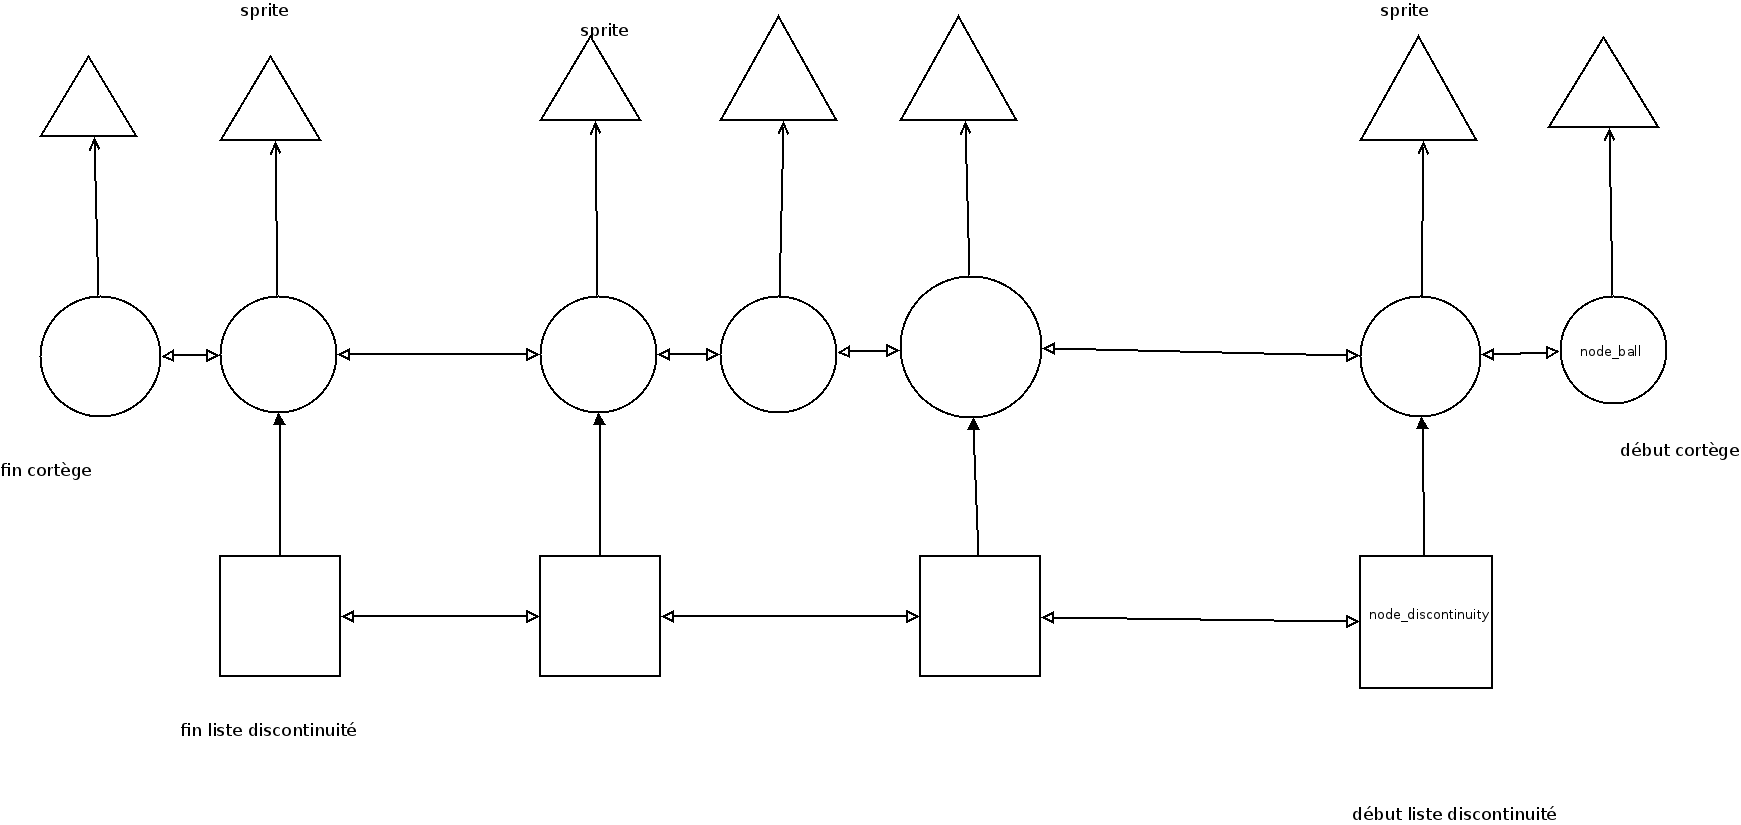
\includegraphics[scale=0.3]{img/discontinuity}

~\\
On détaillera plus tard le mécanisme des discontinuités.


~\\
Du point de vue technique, il est dans un premier temps nécéssaire de metre à jour à intervalle
régulier l'ensemble des données du jeu. Pour cela, on utilise un timer
de la SDL qui à intervalle régulier (16 ms) appele la fonction update 
\textunderscore world. On vera par la suite les problèmes que ce choix pose.
~\\

Le pseudo-code décrivant les grandes lignes de la fonction est le suivant 
\begin{lstlisting}[language=Pascal]

fonction update world()
DEBUT 
Si ((cortege vide OU distance(debut chemin,
queue cortege) > limite ) ET cortege bloque = VRAI ET balles restantes >
0) alors 
       ajouter balle dans cortege
       balles restantes <- balles restantes-1
fin alors

Si cortege vide ET balles restantes = 0 alors
      charger prochain niveau();
fin alors

avancer cortege()
avancer projectile()

fusioner discontinuites()
verifier colision()
verifier projectile()

Si (fin niveau) alors
     Si nombre niveau fait > 1 alors
        sauvegarder score()
     fin alors
fin alors
FIN
\end{lstlisting}
Chacune des fonctions a un certain nombre de paramètre que nous
détaillons pas ici, on se concentre uniquement sur la logique des choses.

~\\
Détaillons chacune des étapes.\\
\textbf{Ajout des boules} \\

On commence par vérifier si on peut ajouter des balles en regardant
s'il en reste ou si le début du chemin n'est pas bloqué par le cortège
arrêté. Ensuite, si ces conditions sont vérifiées, si le cortege est
vide ou si la distance entre le début du chemin et la queue du cortège
est suffisante, on ajoute une balle.

\textbf{Détermination de la longeur suffisante} \\
Nous diposons de boules dont les dimensions sont de 32px par 32px
comme sur le schéma suivant :

\begin{center}
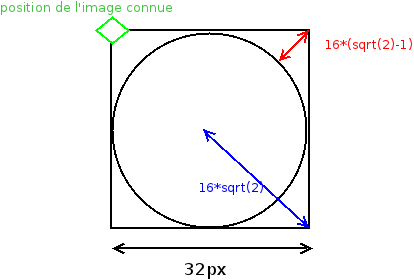
\includegraphics[scale=0.8]{img/boule.png}
\end{center}

En fonction de la position de colision, la distance selon laquelle il
y a choc entre deux boules va varier. Par exemple, si les deux boules
ont même ordonnée, la distance selon laquelle il y aura colision est
de 32px. Par contre, si l'autre boule arrive selon la diagonale, la
distance pour qu'il y ait visuellement choc est de
32-$16(\sqrt{2}-1)$=28 p.x

On définit alors un coefficient (appelé dans le code
COEFF\textunderscore MAGIQUE) qui permet de définir une "colision
moyenne" à 30 px. En disant que la distance entre 2 boules doit être
inférieure à $32*32*COEFF\textunderscore MAGIQUE = 30*30$ pour qu'il y ai
colision, on trouve un coefficient magique de l'ordre de 0.9.
\\
\\
La fonction avancer cortege consite à incrémenter le point courant de
chaque boule du cortège de, de telle sorte que chaque boule voit sa
position augmenter de quelques pixels.
\\
\\
De même, la fonction avancer projectille consiste à augmenter la
position du boulet de en suivant sa loi de
vitesse interne. On ne tient pas compte ici du temps réelement écoulé,
on fait l'hypothèse que la fonction est appelée à une période proche
de 16ms.

~\\
\textbf{Gestion des colisions}
Même si la fusion des discontinuités à lieu avant le gestion des
colisions, regardons comme se gère la gestion des colisions. 

L'idée de départ la fonction est le suivant :


\begin{lstlisting}[language=Pascal]
Pour chaque boule b du cortege faire
  Si distance (projectile,b) < limite alors faire
    balle = inserer dans cortege balle apres b de meme type que projectile
    avancer toutes les boules depuis b jusqu a la tete cortege de 32 points
    nb= nombre total (ie a gauche et a droite de balle) de boules similaires
    Si nb>3 alors  
      on les supprimes du cortege
      on ajoute les boules juste avant et apres a la liste des discontinuite
      Si meme couleur alors
         le cortege avant recule pendant que l arriere s arrete.
      Sinon pas meme couleur, alors
          le cortege avant s arrete pendant que le cortege arriere
            continue d avancer.
      fin si
    sinon 
      ne rien faire
    fin Si
  fin Si
fin faire
\end{lstlisting}

Néanmoins, des modifications d'ordre technique modifient cet
algorithme en différent points. Ces modifications sont détaillées dans
le code.


~\\
\textbf{Gestion des discontinuite}
La gestion des discontinuitées est l'analogue à la gestion des
colisions.
L'idée générale de la fonction est la suivante :
\begin{lstlisting}[language=Pascal]
Pour chaque discontinuite d de la liste faire
  Si distance (d,d->next) < limite alors faire

     retirer d et d->next de la liste

     Si d->val->mouvement = arriere alors
       Pour d a (tete de liste OU d est une discontinuite) faire
           d->val->mouvement= ne pas bouger
       fin faire 
       Pour it=(fin de liste) a  (it tete de liste OU it est une discontinuite) faire
           it->val->mouvement= en avant
       fin faire    
     Sinon si d->val->mouvement = ne rien faire alors

       Pour it= fin de liste a  (it tete de liste OU it est une discontinuite) faire
           it->val->mouvement= en avant
       fin faire         
       
     fin si
  fin Si
fin faire
\end{lstlisting}

\subsection{L'éditeur de niveau}
L'algorithme principal, assez simple, utilisé pour l'éditeur de niveau est le suivant :
\begin{lstlisting}[language=Pascal]
Debut
	si click_droit_appuye
		tantque click_droit_appuye faire
			ecrire_position_souris
		fin tantque
	finsi
fin
\end{lstlisting}
~\\
Les positions sont inscrite dans une liste de points doublement chaînée dans la structure est la suivante :
\begin{lstlisting}
typedef struct list_points list_points;
struct list_points
{
  node_point* head; 	
  node_point* tail;
	/*1 si la liste est finie, 0 sinon*/
	int made;						
  int size;				
	/*Image 5x5 rendant plus visible le trace du parcours*/		
  SDL_Surface *carre;	
	SDL_Surface *ball;	
};
\end{lstlisting}
~\\
Un noeud est ainsi défini :
\begin{lstlisting}
typedef struct node_point node_point;
struct node_point
{
  node_point* next;  	  
  node_point* previous;	
	/*structure contenant x et y*/
  point val;						
};
\end{lstlisting}

~\\La mise en oeuvre de cette algorithme n'a cependant pas été aussi simple. En effet, la gestion de l'événement "MOUSEMOTION" n'étant parfois pas suffisamment rapide, il se peut que les points ne se touchent pas : le chemin tracé est discontinue, 70\% des points manquent.
Une fois la liste terminée, nous utilisons une fonction d'interpolation qui comble ces "trous" par des segments : 
\begin{lstlisting}
/*Fonction qui va combler les discontinuites avec la fonction trace*/
void interpol(list_points* l){ 	
	node_point* it=NULL;
						
	/*Variable temporaire pendant le parcours de a liste*/			
	point temp;									
	it=begin_list_points(*l);		
	
  if(size_list_points(*l)>1){	
	/*On compare tous les points qui se suivent*/	
	while(it->next){
		temp=it->val;
		it=it->next;

		/*Si plus d'un pixel d'ecart on les relie avec trace*/
		if(fabs(temp.x-it->val.x)>1 || fabs(temp.y-it->val.y)>1){
							
		trace(l,temp,it->val);

		}		
	}
 } 
}
\end{lstlisting}

\textbf{Que fait la fonction trace ?}
~\\
On connait le point de départ et celui d'arrivée. On va donc tracer un segment entre les deux et selectionner les pixels le touchant.
Pour cela, avec un paramètre lambda variant entre 0 et 1 on va faire varier un point temporaire sur le segment et incrémenter notre liste de chaque pixel atteint par ce point temporaire.
~\\
\begin{lstlisting}
void trace(list_points* l,point val1,point val2,int* current_pos){ 
  float lambda;
	point temp1=val1;
	point temp2=val1;
	node_point* node;
	for(lambda=0;lambda<=1;lambda+=0.001){

		/*Le point temporaire parcourt le segment*/
		temp1.x=(1-lambda)*val1.x+lambda*val2.x;
		temp1.y=(1-lambda)*val1.y+lambda*val2.y;

		/*On verifie si l'on est passe au pixel suivant*/
    if(fabs(temp1.x-temp2.x)==1 || fabs(temp1.y-temp2.y)==1){

		/*test reussi, on trouve le noeud et on insere*/
		node= find_list_points(*l,temp2);
		insert2_list_points(l,node,temp1);
		temp2=temp1;
		}
  } 
}  
\end{lstlisting}

Cet éditeur qui pouvait parraitre simple à gérer sest finalement avéré être plus compliqué que prévu, à cause de problèmes de discontinuités qu'il nous a fallu résoudre.
\subsection{Les Boutons}
Comme il est très utile d'intéragir avec l'écran via des clicks, nous avons pensé à créer une structure \textbf{bouton} de la manière suivante :
\begin{lstlisting}
/*Pointeur vers une fontion agissant sur state*:
typedef void (*click_handler)(game_state* );

typedef struct bouton bouton;
struct bouton
{	/*La fonction declenchee par le bouton*/
	click_handler on_click;

	/*Le texte qu'affiche le bouton*/
	string text;

	/*Sa couleur*/
	SDL_Color color;
	/*Son etat*/
	int actif;

	/*Position et epaisseur*/
	int x,dx,y,dy;

	/*Style : normal, souligne*/
	int style; 
};
\end{lstlisting}
Indépendamment du bouton, il faudra donc créer des fonctions de type \textbf{click_handler} qui seront appelées si le bouton devient actif.
Cette structure montre son utilité lorsque sur une page il faut créer beaucoup de boutons, on peut alors initialiser chacun d'entre eux par une même fonction utilisant le nombre d'arguments nécessaires, soit 9.
\subsection{Les Scores}
\subsubsection{La strucure}
Pour gérer et garder en mémoire les scores tout au long d'une partie, nous avons constirué la structure \textbf{scores} établie comme suit :
\begin{lstlisting}
typedef struct scores scores;
struct scores
{	/*Le nom du joueur*/
	string name;
	
	/*Le score*/	
	int value;
		
	/*La difficulte*/
	int difficulty; 

	/*Page courante dans le defilement des scores*/
	int page;

	/*Structure de gestion d'evenements localises*/
	bouton* button[5];

	/*Fleches de navigation*/
	SDL_Surface* fleche[4];
}; 
\end{lstlisting} 
Comme toutes les autres, cette structure est associée à des fonctions de création et destruction. Une fois la partie jouée, le score est sauvé dans un des trois fichiers correspondant à chaque difficulté et chacun d'eux sera trié au moment de l'affichage de manière à faire aparaitre les plus élevés en haut.
\subsubsection{La navigation}
Nous avons mis en place un algorithme permettant la navigation dans l'écran des scores suivant la flèche sur laquelle on clique. 
C'est le système de boutons qui nous avons expliqué précédemment, chaque flèche est associé à un bouton dont l'activation avec un click activera la fonction associée : 
\begin{lstlisting}
typedef struct scores scores;
void on_click_gauche(game_state* state){
 /*La difficulte courante baisse ce qui permet d'afficher le tableau associe*/
 state->common_data->score->difficulty--;
 /*On se rammene a la premiere page*/
 state->common_data->score->page = 0;
}
void on_click_droit(game_state* state){
 state->common_data->score->difficulty++;
 state->common_data->score->page = 0;
}
void on_click_haut(game_state* state){
 /*Si on n'est pas sur la premiere page on revient en arriere*/
 if(state->common_data->score->page != 0) state->common_data->score->page--;
}
void on_click_bas(game_state* state){
	state->common_data->score->page++;
\end{lstlisting}
Par suite, dans la fonction display la lecture de cette structure permettra de savoir quelle difficulté afficher via un modulo 3 et quelle page.
\subsection{Les Options}
\subsubsection{La structure}
La structure associée au stockage des options et à l'affichage de celles-ci est la suivante :
\begin{lstlisting}
typedef struct options options;
struct options
{		
 /*boutons des possibilites d'interaction avec l'ecran*/
 bouton* buttons[9];
		
 /*Son actif ou non*/
 int sound;
		
 /*Savoir si le son etait active avant l'affichage*/
 int activ_sound;
   
 /*Choix du theme*/
 int graphic_chosen;
 enum difficulty{easy,medium,hard} diff;

};
\end{lstlisting}
\subsubsection{Interaction avec l'écran}
Chaque click sur l'un de ses boutons(Choix du son, choix de la difficulté, choix du theme, retour au menu) entraîne son activation et donc la mise en route des fonctions associées. Par exemple :
\begin{lstlisting}
void on_click_sound_off(game_state* state){
 if(!(state->common_data->option->buttons[2]->actif)){

 set_button(state->common_data->option->buttons[2],1,TTF_STYLE_UNDERLINE);
 set_button(state->common_data->option->buttons[1],0,TTF_STYLE_NORMAL);
 Mix_PauseMusic();
 state->common_data->option->sound=0;
 save_options(*(state->common_data->option));
	}
}
\end{lstlisting}
La fonction on_click_sound_off soulignera le texte "OFF", mettra la musique en pause, modifiera la structure option et la sauvera dans le fichier texte associé. Finalement la gestion d'événements n'est qu'une boucle qui vériefiera si le click de la souris est sur l'un de ces boutons. 

